\chapter{Bausteinsicht}
\newcommand{\comment}[1]{}

\comment{
	@startuml
	title Middleware-Komponenten – Asynchrones RPC (ohne Anwendung)
	
	package "Client-Middleware" {
		[Client-Proxy]
		[Marshalling]
		[Async RPC Sender]
		
		
	}
	
	package "Middleware Infrastruktur" {
		[Naming Service]
		[Message Transport]
	}
	
	[Client-Proxy] --> [Naming Service] : Dienstadresse auflösen
	[Client-Proxy] --> [Marshalling] : Argumente serialisieren
	[Marshalling] --> [Async RPC Sender] : Anfrage senden
	package "Server-Middleware" {
		[Async RPC Receiver]
		[Unmarshalling]
		[Server-Skeleton]
		
		[Async RPC Receiver] --> [Unmarshalling] : Deserialisieren
		[Unmarshalling] --> [Server-Skeleton] : Methodenaufruf
	}
	
	
	[Async RPC Sender] --> [Message Transport]
	[Message Transport] --> [Async RPC Receiver]
	@enduml
}

\begin{figure}[htbp]
	\centering
	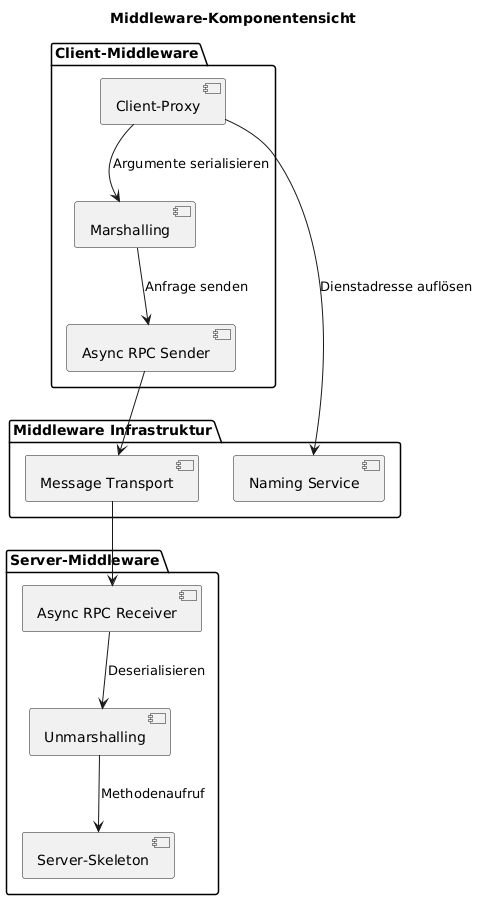
\includegraphics[width=0.8\textwidth]{diagrams/bausteinsicht.png}
	\caption{Komponenten der Middleware}
	\label{fig:meine-abbildung}
\end{figure}


\section*{Beschreibung}